% !TeX root = ../main.tex
% Add the above to each chapter to make compiling the PDF easier in some editors.

\chapter{Implementation}\label{chapter:implementation}
Building on the framework architecture explained in Chapter \ref{chapter:Approach}, we describe the middleware proof-of-concept (POC) implementation in details to show that the framework architecture is sound. Moreover we describe the flows implementation used to create the use cases in order tp provide the evaluation for the framework. \\

\section{Middleware}

 The middleware is written in Java, it uses Maven as a  software project dependency management which handles the middleware build. Maven projects contain a Project Object Model (POM) file which describes the dependencies and libraries used by the project. In addition, it has build configuration management that is used to build the project and create a runnable jar file. The middleware can be compiled and packaged to a jar using the following command \verb|mvn clean package|. The project contains dependencies for \textit{Lombok} which is a library that generates getters, setters and constructors during compile time without the need to write them in the Java classes, \textit{Gson} dependency in order to be able to read and write in JSON format, \textit{SCAMPI API} which allows us to publish, subscribe and override some functions from SCAMPI, dependencies to create a web application through \textit{Spring Boot}. \\
 
 \noindent The project is divided into several packages, we describe them in alphabetical order, the package \verb|com.middleware.api| which contains two classes, \verb|SCAMPApi.java|  and \verb|MiddlewareApi.java|. As shown in \ref{fig:cd-api}, the class \verb|SCAMPIAPI.java| implements two classes for the SCAMPI server which includes functions like \verb|OnConnected()|, \verb|OnDisconnected()|, \verb|OnConnectedFailed()|, \verb|OnStopped()| and \verb|messageReceived()|. It also contains a cache for messages and a field indicating the machine specification
  
 \begin{figure}[H]
 	\centering
 	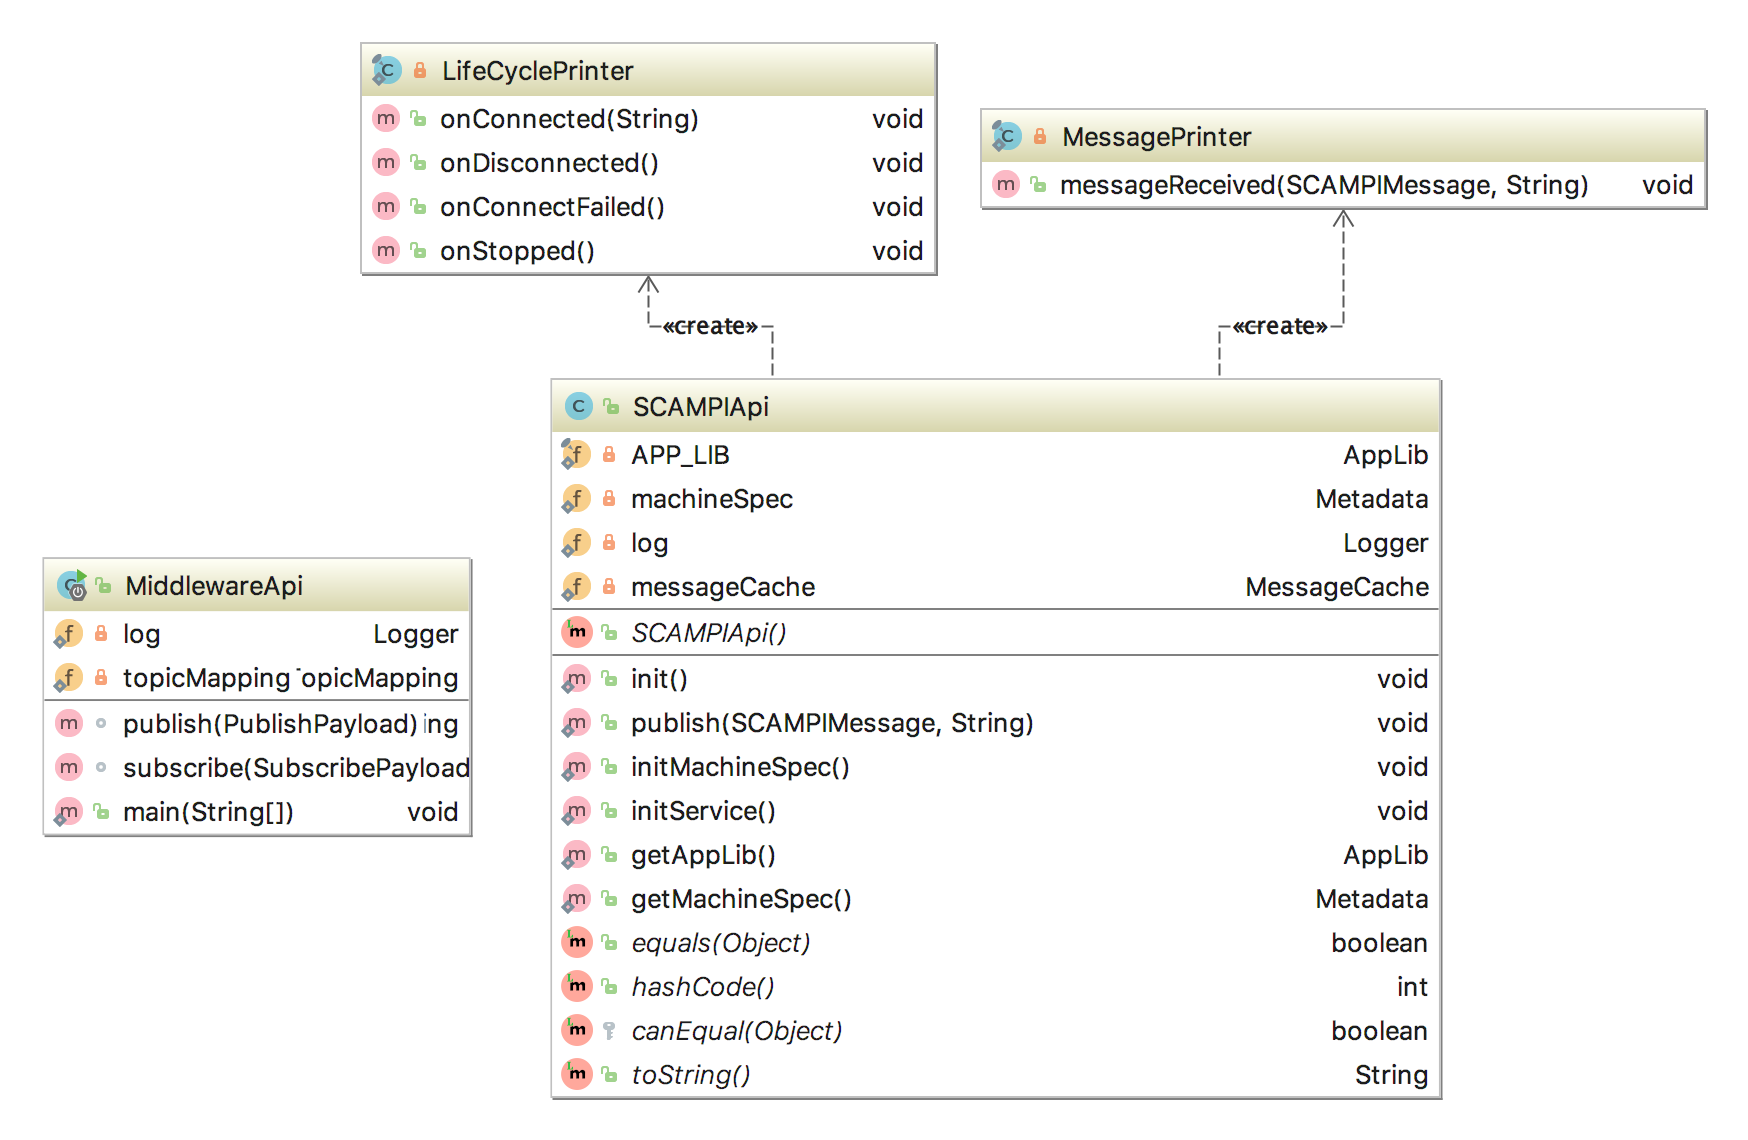
\includegraphics[scale=0.2]{images/cd-api.png}
 	\caption{Class diagram for the api package. }
 	\label{fig:cd-api}
 \end{figure}
 
 \noindent The third packages is called \verb|com.middleware.constants| and has one class \verb|Constants.java| which contain all the constant fields used in the middelware across all other classes. This includes string keys for SCAMPI messages, some linux commands,  URL for the local node-RED instance, path for user home directory and path for the JSON file that includes the machine specification.ß
 
 \begin{figure}[H]
 	\centering
 	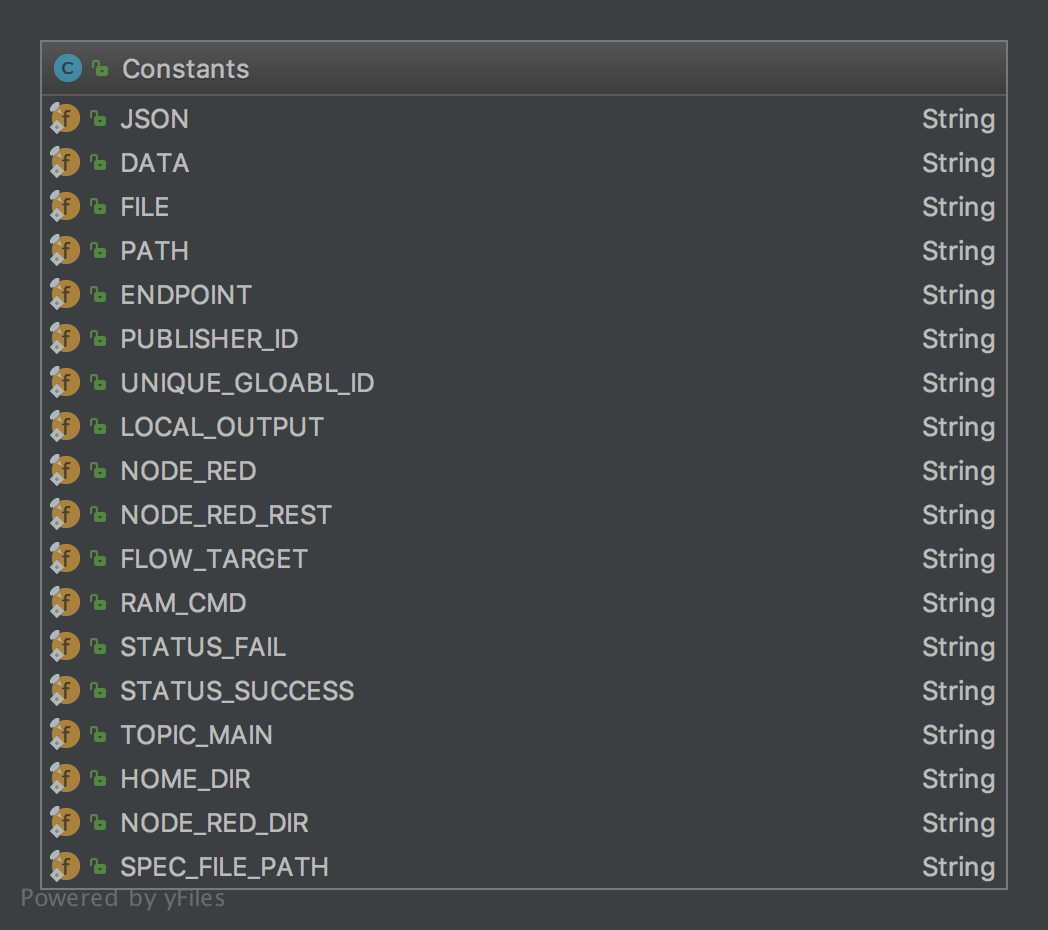
\includegraphics[scale=0.18]{images/constants.png}
 	\caption{Class diagram for the constants class. }
 	\label{fig:cd-constants}
 \end{figure}


